\documentclass{article}

\usepackage[english]{babel}
\usepackage[utf8]{inputenc}
\usepackage{amsmath,amssymb}
\usepackage{parskip}
\usepackage{graphicx}
\usepackage{listings}
\usepackage{float}

% Margins
\usepackage[top=2.5cm, left=3cm, right=3cm, bottom=4.0cm]{geometry}
% Colour table cells
\usepackage[table]{xcolor}

% Get larger line spacing in table
\newcommand{\tablespace}{\\[1.25mm]}
\newcommand\Tstrut{\rule{0pt}{2.6ex}}         % = `top' strut
\newcommand\tstrut{\rule{0pt}{2.0ex}}         % = `top' strut
\newcommand\Bstrut{\rule[-0.9ex]{0pt}{0pt}}   % = `bottom' strut

%%%%%%%%%%%%%%%%%
%     Title     %
%%%%%%%%%%%%%%%%%
\title{CSCI803 Assignment}
\author{Yao Xiao \\ SID 2019180015}
\date{\today}

\begin{document}
\maketitle

%%%%%%%%%%%%%%%%%
%   Problem 1   %
%%%%%%%%%%%%%%%%%
\section{Problem 1}
\subsection{Part 1}
\begin{enumerate}
    \item The first stage is to identify the problem and thoroughly understand it, After obtaining the input, break out the problem into stages and calculate what happens at each step so the next step can occur.
    \item The second stage is to start anlyzing how efficient the code is in solving the problem after obtaining the basic framework of the algorithm, the biggest problem here is deciding when the algorithm has reached maximum efficiency for the project and produces acceptable results. 
    \item The third stage is to write and code the algorithm, and in order to know how to write the algorithm efficiently, the developer should know exactly what each line of codes is going to accomplish when the program is executed.
    \item Once the algorithm is designed and coded go back and experiment with different variables in the algorithm, when finding flaws in what you have written or ways to write the code better, then go back to the design step and redesign the algorithm.
\end{enumerate}

Actually, the design and analysis of the algorithm is a cyclical process.
And experimentation with existing algorithms may lead to new designs.

\subsection{Part 2}
Analysis of algorithms means to investigate an algorithm’s
efficiency with respect to resources: running time and memory space.

Both time and space efficiencies are measured as functions of input
size. Time efficiency is measured by counting the number of basic
operations executed in the algorithm. The space efficiency is
measured by the number of extra memory units consumed.
The framework’s primary interest lies in the order of growth of the
algorithm’s running time (space) as its input size goes infinity.
The efficiencies of some algorithms may differ significantly for
inputs of the same size. For these algorithms, we need to distinguish
between the worst-case, best-case and average case efficiencies.

\subsection{Part 3}
Asymptotic notations are the mathematical notations used to describe the running time of an algorithm when the input tends towards a particular value or a limiting value. For example: In bubble sort, when the input array is already sorted, the time taken by the algorithm is linear i.e. the best case.

\section{Problem 2}

\begin{enumerate}
    \item $O(t(n)) = O(n^2)$
    \item $log(3n+4/n) = log[(3n^2+4)/n] = log(3n^2+4) - logn = 2logn - logn = logn$, so Big O belongs to O(n)
\end{enumerate}


\section{Problem 3}
\begin{lstlisting}
def binary_search(find, raw_list):
    low = 0
    high = len(raw_list) - 1
    while low <= high:
        mid = (low + high) // 2
        if raw_list[mid] == find:
            return mid
        elif raw_list[mid] > find:
            high = mid - 1
        else:
            low = mid + 1
    return -1


raw_list = [1, 3, 8, 12, 23, 28, 37, 40, 48, 66]

raw_list.sort()

print("Origin list:", raw_list)
try:
    find = int(input("Please input key:"))
except:
    print("Please input integer")
    exit()

result = binary_search(find, raw_list)
if result != -1:
    print("The element is %d and its number is %d" % (find, result))
else:
    print("Cannot find!")
\end{lstlisting}

\subsection{Output}
\begin{figure}[H]
    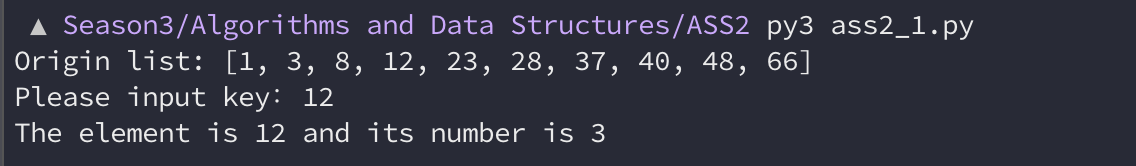
\includegraphics[width=1\textwidth]{Fig1.png}
\end{figure}

\subsection{Analysis}
\begin{itemize}
    \item Best Case - O(1), it is when the middle element is the target.
    \item Average Case - O(logn)
    \item Worst Case - O(logn), many situations like when the target item is not in the search list making $\lfloor log_2(n)+1 \rfloor$ iterations.
    \item Binary search requires three pointers to elements, which may be array indices or pointers to memory locations, regardless of the size of the array. Therefore, the space complexity of binary search is O(1).
\end{itemize}

\section{Problem 4}
\begin{lstlisting}
def is_prime(n):
    if n == 1:
        return False
    i = 2
    while i * i <= n:
        if n % i == 0:
            return False
        i += 1

    return True


for x in range(1, 11):
    print('%d: %s' % (x, is_prime(x)))

print('%d: %s' % (10000000, is_prime(1000000000)))

print('%d: %s' % (10000005, is_prime(1000000007)))
\end{lstlisting}

\subsection{Output}
\begin{figure}[H]
    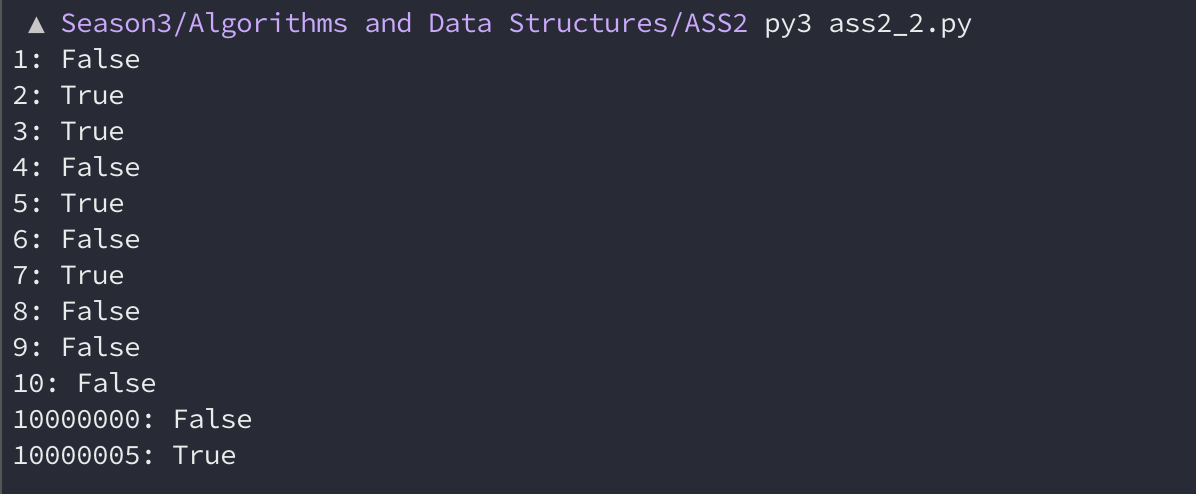
\includegraphics[width=1\textwidth]{Fig2.png}
\end{figure}

\subsection{Analysis}
\begin{itemize}
    \item Time Complexity of the above algorithm is O(sqrt(n)).
    \item Space Complexity of the above algorithm is O(1).
\end{itemize}

\end{document}
